% ICICPE 2026 - When More Detections Hurt: detector confidence and gating in a
% modernized DeepSORT pipeline. Template: ICICPE custom (icicpe.sty).
% Named (final-copy) submission.

\documentclass[twocolumn, 10pt]{article}

\usepackage{icicpe}
\usepackage[utf8]{inputenc}
\usepackage[pdfencoding=auto,hidelinks]{hyperref}
\usepackage{url}
\usepackage{amsmath}
\usepackage{amssymb}
\usepackage{latexsym}
\usepackage{graphicx}
\usepackage[symbol]{footmisc}
\usepackage{booktabs}
\usepackage[capitalize,noabbrev]{cleveref}
\usepackage{tikz}
\usetikzlibrary{positioning,arrows.meta,calc,fit,backgrounds}

\DeclareMathOperator*{\argmax}{arg\,max}
\DeclareMathOperator*{\argmin}{arg\,min}

% Numerical macros (final values substituted from the gating study;
% see paper/experiments/analyze.py and results_macros.tex).
% Numeric results. The six-video headline and the gating sweep come from one controlled
% run (paper/experiments/gating_study.csv, imgsz 1280); analyze.py fills the sweep summary.

% --- headline: six-video mean HOTA (controlled study) ---
\newcommand{\baselineHOTA}{40.17}        % original DeepSORT (provided detections + mars)
\newcommand{\modernDefaultHOTA}{49.27}   % modern, ungated default gate (conf 0.25)
\newcommand{\modernHOTA}{52.96}          % modern, gated (conf 0.45) -- beats baseline on all six
\newcommand{\modernBestHOTA}{53.27}      % modern, per-clip best gate
\newcommand{\deltaHOTA}{12.79}           % gated minus baseline
\newcommand{\deltaDefaultHOTA}{9.10}     % default minus baseline
\newcommand{\fpsRealtime}{9.87}

% --- detection-vs-association decomposition (MOT16 split, default configuration) ---
\newcommand{\detaGain}{+12.30}
\newcommand{\assaGain}{+6.25}
\newcommand{\baselineMOTA}{46.34}
\newcommand{\modernMOTA}{46.75}

% --- REID-only under ground-truth boxes (association isolated) ---
\newcommand{\osnetGT}{89.93}
\newcommand{\timmGT}{89.22}
\newcommand{\osnetainGT}{87.33}

% --- OSNet vs timm in the full live pipeline (real detections, course journal) ---
\newcommand{\osnetReal}{52.54}
\newcommand{\timmReal}{47.70}
\newcommand{\reidRealGap}{4.84}

% --- TUD-Campus levers (controlled study) ---
\newcommand{\imgszLow}{39.65}      % imgsz 960  (conf 0.25)
\newcommand{\imgszMid}{35.03}      % imgsz 1280 (conf 0.25, the default)
\newcommand{\imgszHigh}{29.75}     % imgsz 1536 (conf 0.25)
\newcommand{\tudUntuned}{4.83}     % magnitude: default gate (conf 0.25) below baseline on TUD-Campus
\newcommand{\tudGain}{6.44}        % magnitude: gated (conf 0.45) above baseline on TUD-Campus

% --- six-video confidence sweep summary (filled by analyze.py) ---
\newcommand{\nVideos}{6}
\newcommand{\nHurt}{6}             % videos where conf 0.45 net-beats conf 0.15 (endpoint test in analyze.py)
\newcommand{\corrPearson}{-0.90}   % corr( per-clip precision , HOTA gained by raising the gate )
\newcommand{\ablationRecover}{+2.57}


\title[english]{When More Detections Hurt: A Controlled Audit of Detector\\
       Confidence and Gating in a Modernized DeepSORT Pipeline}

\author[english]{
Sergei Solovev \\
HSE University \\
\texttt{sesesolovev@edu.hse.ru} \\
}

\finalcopy

\begin{document}

\twocolumn[
\maketitle
\begin{abstract}
Modernizing a 2017-era DeepSORT tracker by swapping its precomputed detections and fixed appearance
encoder for a contemporary detector (YOLOv8m) and re-identification model (OSNet) raises mean HOTA on
six MOT-Challenge videos from \baselineHOTA{} to \modernHOTA{} ($+\deltaHOTA$). \textbf{This headline
gain is unsurprising and unpublishable on its own; the contribution of this paper is the audit
underneath it.} First, the gain is \textbf{detection-dominated}: on the MOT16 split the detection
term rises by $\detaGain$ HOTA points against only $\assaGain$ for the association term, and under
ground-truth boxes a generic ImageNet backbone (not trained for re-identification) reaches
\timmGT{} HOTA versus \osnetGT{} for a dedicated OSNet, so association quality is nearly
detector-bound once detection is fixed. Second, the mean hides a regression: at its default gate the
modernized tracker scores below the 2017 baseline on the least-precise clip (TUD-Campus, $35.0$ vs.\
$39.9$ HOTA). We trace this to a counterintuitive regime: across \textbf{all six videos, lowering the
detector confidence gate (admitting more low-confidence detections) never raises and usually lowers
HOTA}, and the size of the penalty tracks per-clip detector precision (Pearson $r = \corrPearson$).
The cause is specific and reproducible: the modern live pipeline drops the original DeepSORT confidence
and non-maximum-suppression gate, so ungated false positives spawn spurious tracks; a
gating-restoration ablation recovers the loss, and raising the per-clip confidence threshold lifts the
worst sequence from a $\tudUntuned$-point deficit to $+\tudGain$ over baseline. We connect this to
ByteTrack, which keeps low-confidence detections but associates rather than instantiates them, and
argue that in tracking-by-detection \textbf{per-clip precision gating is a larger and more reliable
lever than global recall maximization}. We additionally report environment-driven negative results
(NumPy-2.x dependency breakage; a ground-truth-format bug that silently zeroed four sequences) as
reproducibility lessons.
\end{abstract}

\begin{keyword}
multi-object tracking, tracking-by-detection, DeepSORT, HOTA, detector confidence,
non-maximum suppression, gating, person re-identification, MOT-Challenge
\end{keyword}
]

\section{Introduction}
\label{sec:intro}

Multi-object tracking is dominated by the tracking-by-detection paradigm: a per-frame object detector
proposes boxes, and an association stage links them across time into identity-consistent tracks. DeepSORT
\cite{wojke2017deepsort}, which augments the SORT core \cite{bewley2016sort} (a Kalman filter plus
Hungarian assignment) with a deep appearance embedding, remains a canonical instance of this design and a
common baseline. Its original detector and re-identification (re-ID) encoder are now nearly a decade old, so
the engineering instinct is obvious: swap in a contemporary detector and a modern re-ID backbone behind the
unchanged SORT core. We do exactly this, integrating pluggable detectors (YOLOv8m \cite{jocher2023yolov8})
and re-ID models (OSNet \cite{zhou2019osnet}; a generic ImageNet timm backbone \cite{wightman2019timm})
through a single \texttt{Detection(tlwh, confidence, feature)} contract. On six MOT-Challenge training videos
\cite{leal2015mot15,milan2016mot16}, mean HOTA \cite{luiten2021hota,luiten2020trackeval} rises from
\baselineHOTA{} to \modernHOTA{} ($+\deltaHOTA$) at \fpsRealtime{} FPS. This headline result is also
unsurprising and, on its own, unpublishable: a stronger detector and a stronger encoder make a better
tracker.

The interesting questions are the ones the headline number hides. \emph{Where} does the gain actually come
from -- the better detector, or the better appearance model? And does a stronger detector always help: can
\emph{more} detections, obtained by raising recall, ever \emph{hurt} tracking quality? We find that the
answers are not the intuitive ones. The modernization gain is overwhelmingly detection-driven, and on dense,
low-resolution clips pushing the detector toward higher recall drives HOTA monotonically \emph{down}. The
mechanism is concrete and reproducible: the modern live pipeline silently drops the original DeepSORT gating
contract (a $0.3$ confidence threshold plus non-maximum suppression) that once filtered the precomputed
detections, so ungated false positives instantiate spurious tracks. This leads to our thesis:
\textbf{in tracking-by-detection, per-clip detector-confidence (precision) gating is a larger and more
reliable lever on HOTA than global recall maximization}.

We make four contributions.
\begin{enumerate}
\item A detection-vs-association decomposition of the modernization gain, showing it is
\textbf{detection-dominated}: on MOT16 the detection term improves by $\detaGain$ HOTA against only
$\assaGain$ for association, and under ground-truth boxes a non-re-ID-trained ImageNet backbone reaches
\timmGT{} HOTA versus \osnetGT{} for a dedicated re-ID model, so association is nearly detector-bound once
boxes are fixed.
\item A counterintuitive \textbf{``more detections hurt''} regime on dense low-resolution clips: raising the
TUD-Campus input resolution lowers HOTA monotonically
($\imgszLow\!\rightarrow\!\imgszMid\!\rightarrow\!\imgszHigh$), and the sign of recall's effect is predicted
by per-clip detector precision across all \nVideos{} videos.
\item A gating-restoration ablation that attributes the regression to the dropped confidence and NMS gate
and recovers the loss.
\item A practical \textbf{per-clip precision-gating guideline}: tuning the confidence threshold per clip
lifts the worst sequence from a $\tudUntuned$ deficit to $+\tudGain$ HOTA over baseline.
\end{enumerate}

We position this finding against ByteTrack \cite{zhang2022bytetrack} and other modern DeepSORT descendants
\cite{du2023strongsort,cao2023ocsort,aharon2022botsort} in \cref{sec:related}, detail the system and
protocol in \cref{sec:method}, report the audit in \cref{sec:results}, and discuss limitations and
reproducibility lessons in \cref{sec:limitations} before concluding.

\section{Background and Related Work}
\label{sec:related}

\subsection{SORT, DeepSORT, and the Gating Contract}

Tracking-by-detection casts multi-object tracking as per-frame detection followed by frame-to-frame data association. SORT \cite{bewley2016sort} pairs a constant-velocity Kalman filter with greedy Hungarian assignment on intersection-over-union, prioritizing speed. DeepSORT \cite{wojke2017deepsort} augments this core with a learned appearance descriptor and a cosine-distance gate \cite{wojke2018cosine}, reducing identity switches under occlusion. Across both, the association core -- prediction, Hungarian matching, and the appearance gate -- is the component most often credited with tracking quality.

Less discussed, but central to this work, is that the original DeepSORT does not consume raw detections directly. Its public pipeline~\cite{wojke2017deepsortcode} applies an explicit \emph{gating contract} to the precomputed detection set before any of them reach the tracker: detections below a confidence threshold (\texttt{min\_confidence} $=0.3$) are discarded, boxes below a minimum height are removed, and per-frame non-maximum suppression (NMS) prunes overlapping responses. Only the survivors are wrapped as \texttt{Detection(tlwh, confidence, feature)} objects and passed to \texttt{predict()}/\texttt{update()}. This filter is a precision-oriented admission policy: it trades recall for a cleaner detection stream, suppressing the low-confidence and duplicate boxes that would otherwise instantiate spurious tracks. Modernization efforts that swap in a contemporary detector behind the same association core can silently \textbf{drop this gate}, since the new detector is typically queried in a streaming, ungated fashion; our audit shows this omission, rather than the association core, drives the most consequential behavior on dense clips.

\subsection{HOTA and the DetA/AssA Decomposition}

We evaluate with Higher Order Tracking Accuracy (HOTA) \cite{luiten2021hota} via TrackEval \cite{luiten2020trackeval}. HOTA's appeal here is structural: it factorizes geometrically into a detection term and an association term, $\mathrm{HOTA} \approx \sqrt{\mathrm{DetA} \cdot \mathrm{AssA}}$, where DetA scores how well predicted boxes localize ground-truth objects and AssA scores how consistently identities are maintained across the matched detections. This decomposition lets us attribute a change in tracking quality to detection versus association rather than reading a single conflated number, which is precisely the lever our study exercises: a modernization gain or a regression can be assigned to the DetA or the AssA factor, and a precision change in the detection stream registers directly in DetA. Earlier scalar metrics such as MOTA conflate these effects and weight identity errors lightly, obscuring the detection-driven regime we report. This detection-dominated regime is documented in the work that motivates HOTA. Luiten et al.~\cite{luiten2021hota} show that for the top MOT17 trackers detection error accounts for almost all of the variance in the legacy MOTA score (a linear fit gives $R^2 \approx 0.99$ against the detection term versus $R^2 \approx 0.24$ against the association term, with the detection-to-association error ratio ranging from roughly $42$ to $186$), the very imbalance HOTA was designed to correct. The dominance persists in modern systems: ByteTrack~\cite{zhang2022bytetrack} reaches strong accuracy with no appearance model at all, and StrongSORT~\cite{du2023strongsort} attributes more of its gains to a stronger detector than to its appearance and association refinements. An equal-magnitude change in the detection stream therefore moves the score more than a comparable association change -- the premise our decomposition (\cref{sec:decomp}) tests directly.

\subsection{ByteTrack and the Gating Mechanism}

ByteTrack \cite{zhang2022bytetrack} is the natural point of comparison, since it too revisits how low-confidence detections are handled, but its mechanism is the opposite of an admission gate and must be positioned carefully. ByteTrack \emph{keeps} low-confidence boxes rather than thresholding them away; crucially, it uses them only in a second association pass to recover \emph{existing} tracks, and never lets a low-confidence box \emph{instantiate} a new track (new tracks are seeded only from the remaining high-confidence detections, so ByteTrack already embodies a precision gate for instantiation). Our finding concerns ungated low-confidence detections that are free to spawn spurious new tracks, inflating identity counts and false positives on dense scenes. These are complementary mechanisms operating on the same raw material: ByteTrack constrains where weak detections may act (association only), whereas the dropped DeepSORT contract constrained whether they enter at all. ByteTrack is therefore not a counterexample to our result but an instance of the same underlying principle -- weak detections must be admitted under restriction -- realized at a different stage of the pipeline.

\subsection{Modern DeepSORT Descendants}

A family of trackers extends the DeepSORT design. StrongSORT \cite{du2023strongsort} upgrades the appearance model, motion compensation, and feature update; OC-SORT \cite{cao2023ocsort} reworks the motion model to be observation-centric and robust to nonlinear motion and occlusion; BoT-SORT \cite{aharon2022botsort} adds camera-motion compensation and a fused IoU--appearance cost. The lineage has continued through 2024--2025 along axes orthogonal to track admission: Deep OC-SORT \cite{maggiolino2023deepocsort} folds adaptive appearance and camera-motion compensation into the OC-SORT association cost, UCMCTrack \cite{yi2024ucmctrack} replaces IoU with a ground-plane Mahalanobis distance under uniform camera-motion compensation, and Hybrid-SORT \cite{yang2024hybridsort} fuses detector confidence, box height, and velocity direction as additional weak cues. These advances target the association core, and they generally inherit a confidence threshold as a fixed hyperparameter rather than treating it as the dominant, scene-dependent lever.

Crucially, the admission and track-initialization gate is not absent from these descendants; it is instantiated as an explicit, separately tuned hyperparameter. ByteTrack \cite{zhang2022bytetrack} seeds new tracks only from unmatched high-confidence detections, with the birth threshold set above its association threshold; BoT-SORT \cite{aharon2022botsort} exposes the same decision as a first-class \texttt{new\_track\_thresh}; OC-SORT \cite{cao2023ocsort} spawns tracklets only from detections passing a \texttt{det\_thresh}; and StrongSORT \cite{du2023strongsort} inherits DeepSORT's confidence gate (\texttt{min\_confidence}) and temporal confirmation gate (\texttt{n\_init}). Our contribution is therefore not the discovery that gating matters -- the field already treats the gate as a named, tuned parameter -- but the audit of a routine modernization in which this otherwise-explicit gate is silently dropped, together with a per-clip, precision-dependent quantification of what the omission costs. The per-clip precision-gating insight is in this sense orthogonal and composable: it does not compete with the association improvements above but specifies how the detection stream feeding any of them should be admitted, and is most decisive exactly where their motion and appearance machinery has the least to work with -- dense, low-resolution clips with unreliable detections.

A parallel line treats detection confidence as an actively engineered lever rather than a fixed threshold. BoostTrack \cite{stanojevic2024boosttrack} and BoostTrack++ \cite{stanojevic2025boosttrackpp} compute a detection--tracklet confidence score and use it to boost or reweight detections so that more genuine objects are admitted, while Localization-Guided Track \cite{meng2023lgtrack} decomposes detection confidence into classification and localization components to choose the association cost rather than discarding low-confidence boxes uniformly. That such effort is spent deliberately engineering confidence handling underscores how consequential the admission policy is, and how readily a naive modernization can mishandle it.

A complementary family, joint-detection-and-embedding trackers such as JDE \cite{wang2020jde} and FairMOT \cite{zhang2021fairmot}, learns detection and appearance together, arguing that anchor-based detection otherwise corrupts the re-identification features trained alongside it; our ground-truth-box isolation does not contradict this position, since it measures the descriptor's marginal value with detection \emph{held fixed} rather than claiming appearance is unimportant in general.

\subsection{ImageNet Features as a Re-identification Baseline}

Finally, generic ImageNet-pretrained features are a well-established re-identification baseline, routinely reported as the lower anchor that purpose-built descriptors such as OSNet \cite{zhou2019osnet} (here via torchreid \cite{zhou2019torchreid}) must clear. Our near-parity result between a non-REID-trained timm backbone \cite{wightman2019timm} and OSNet is therefore \emph{not} a claim that ImageNet features rival dedicated REID models in general. It is a controlled isolation: under ground-truth boxes the detection stage is held fixed, removing detector-induced variance so that association quality is measured directly, and in that regime the two appearance models are nearly indistinguishable on these short sequences. We report it to quantify how little of the modernization gain is attributable to the appearance descriptor once detection is controlled for, reinforcing the detection-dominated decomposition that motivates the rest of the paper.

\section{System and Experimental Protocol}
\label{sec:method}

\subsection{Modernized Pluggable System}

We modernize the reference DeepSORT implementation \cite{bewley2016sort,wojke2017deepsort}
along exactly two axes -- detection and appearance -- while leaving the tracking core untouched.
The original codebase consumes \emph{precomputed} detections from disk and a fixed appearance
encoder. We replace both with pluggable, swappable adapters selected by name at run time: a
detector front-end and a re-identification (REID) front-end, each registered through a small
registry so a tracker is specified as a (detector, REID) pair. In this paper the detector is
YOLOv8m \cite{jocher2023yolov8} and the REID model is either OSNet \cite{zhou2019osnet} (trained
for person re-identification) or a generic ImageNet \texttt{timm} backbone \cite{wightman2019timm}
(\emph{not} trained for re-identification), used as a deliberately weak appearance baseline.

The SORT core is preserved verbatim: an 8-dimensional constant-velocity Kalman filter, Hungarian
assignment, and a cascaded matcher that combines a Mahalanobis motion gate with a cosine
\emph{appearance} gate over REID descriptors. Its track lifecycle (confirmation after $n_{\text{init}}$
hits, deletion after $\text{max\_age}$ misses) is unchanged. The integration contract between the
modern front-ends and this core is a single value object: each detection is a
\texttt{Detection(tlwh, confidence, feature)} -- a top-left/width-height box, a scalar detector
confidence, and an appearance vector -- and the per-frame loop is the original
\texttt{tracker.predict()} followed by \texttt{tracker.update(detections)}. Because the contract and
the core are fixed, any change in tracking quality is attributable to the detector, the REID model,
or the pre-tracker \emph{gating} that decides which detections reach \texttt{update()}.

\paragraph{The dropped gate.}
This last point is central. In the original pipeline, precomputed detections passed through a fixed
gate before reaching the tracker~\cite{wojke2017deepsortcode}: a confidence threshold
($\text{min\_confidence}$), a non-maximum-suppression (NMS) step on overlapping boxes, and a minimum
box-height filter. The
modern live pipeline runs the detector \emph{inside} the loop, and its default configuration
\textbf{drops this gate}: $\text{min\_confidence}=0.0$ and $\text{nms\_max\_overlap}=1.0$, which
disables both the confidence filter and the secondary NMS (on the assumption that the detector's own
internal NMS and \texttt{conf} threshold suffice). Every YOLO detection above the detector's own
low internal threshold is therefore lifted directly into a \texttt{Detection} and offered to the
tracker. This single configuration change -- not any change to the Kalman filter or the matcher -- is
the regression we audit in \cref{sec:results}: ungated low-confidence boxes are free to instantiate
spurious new tracks. The gate itself is still present in the code path (the same confidence-filter-plus-NMS
gate as the reference pipeline~\cite{wojke2017deepsortcode}), merely disabled by default, which makes the
restoration ablation below a one-line configuration change rather than a code change.

\subsection{Evaluation Protocol}

We evaluate on six MOT-Challenge training sequences spanning two benchmarks: TUD-Campus,
TUD-Stadtmitte, KITTI-17, and PETS09-S2L1 from 2D MOT 2015 \cite{leal2015mot15}, and MOT16-09 and
MOT16-11 from MOT16 \cite{milan2016mot16}. The set deliberately mixes clean, sparse scenes with
dense, low-resolution ones, since per-clip density is the axis along which our central effect
reverses sign. The primary metric is HOTA \cite{luiten2021hota}, computed by the official TrackEval
toolkit \cite{luiten2020trackeval}; we report its DetA and AssA sub-scores when decomposing detection
versus association. End-to-end throughput, timed on one sequence (MOT16-09), is \fpsRealtime{}~FPS
(detection and re-identification each run near $30$~FPS; their serial composition is the bottleneck).

\subsection{Controlled Experimental Design}

The experiments are designed so that each varies one lever while holding the others fixed.

\paragraph{(a) Detection-vs-association decomposition (GT-box, REID-only).}
To separate the modernization gain into a detection component and an association component, we run a
\emph{ground-truth-box} mode in which the detector is replaced by an oracle that emits the ground-truth
boxes, with the confidence/NMS gate skipped. Detection is then perfect and identical across runs, so
the only free variable is the REID model feeding the appearance gate. Comparing OSNet against the
\texttt{timm} backbone in this mode (\osnetGT{} vs.\ \timmGT{} HOTA) isolates how much association
quality the appearance model contributes once detection is held perfect; comparing the same models in
the full pipeline against this ceiling reveals how detector-bound association quality is in practice.

\paragraph{(b) Per-video detector-confidence sweep.}
For each of the six videos we sweep the YOLO confidence threshold over
$\{0.15, 0.25, 0.35, 0.45\}$, holding the detector, REID model, input size, and SORT core fixed. This
is the precision/recall lever: lowering the threshold raises recall and lowers precision. We pair the
HOTA response with the detector's per-clip precision at conf~0.25 to test whether the \emph{magnitude}
of recall's effect on HOTA is predicted by per-clip precision.

\paragraph{(c) Input-size sweep on the two dense clips.}
On the two dense, low-resolution clips (TUD-Campus and KITTI-17), where YOLO precision is low, we
additionally sweep the detector input resolution over $\{960, 1280, 1536\}$ (the $1280$ midpoint is the
default configuration, shared with the confidence sweep). Larger input recovers
more small instances -- a second, \emph{orthogonal} recall lever to the confidence threshold -- and
lets us test whether it reproduces the confidence-sweep effect or, by changing \emph{which} detections
exist rather than merely gating them, behaves differently.

\paragraph{(d) Gating-restoration ablation.}
To attribute the regression specifically to the dropped gate, we restore a DeepSORT-style admission
gate -- the reference reproduction value $\text{min\_confidence}=0.3$~\cite{wojke2017deepsortcode}
together with secondary NMS at overlap~$0.7$ (our setting; the reference default is $1.0$) -- on top of
the otherwise unchanged modern pipeline, and re-measure HOTA on each video. Because the gate acts only
on the detection stream feeding the unchanged tracker, any recovered HOTA is causally attributable to
admission, not to a confounding code change.

\paragraph{Reproducibility.}
The detector is pinned: ultralytics~8.4.79 with the \texttt{yolov8m.pt} checkpoint
(sha256 \texttt{5d4a90cd\dots4fe5}) at input size~1280. Per-clip detector precision is
weight-version-sensitive, so we fix and report the version; a different ultralytics release
shifts the absolute values (e.g.\ TUD-Campus precision $0.50$ rather than $0.43$) but leaves the
low-precision ordering -- TUD-Campus and KITTI-17 lowest -- on which the analysis depends unchanged.
Every run -- each detector preset, REID model, confidence level, input size, and ablation -- appends
one row to a versioned CSV journal recording the configuration and resulting metrics, so the full
experimental history is traceable and the gating-sweep figures in \cref{sec:results} (confidence,
precision, input-size, and ablation plots) are regenerable from it; the decomposition and
ground-truth-box numbers come from separate evaluation runs recorded in the same journal. The
sweep harness writes each result immediately and skips configurations already present, so an
interrupted run resumes without recomputation. We also note two environment-level pitfalls that the
journal helped surface and that we report as negative results in \cref{sec:limitations}: a NumPy-2.x
incompatibility that breaks the torchreid/boxmot/TrackEval build chain, and a 2D~MOT~2015-vs-MOT16
ground-truth column-format mismatch that silently zeroed four sequences until corrected.

\section{Results}
\label{sec:results}

\subsection{Where the Gain Comes From}
\label{sec:decomp}

The modernized tracker (YOLOv8m + OSNet) raises mean HOTA from \baselineHOTA{} to \modernHOTA{}
($+\deltaHOTA$) and exceeds the baseline on every one of the six videos (\cref{tab:fullpipeline}).
Decomposing the gain on the combined MOT16 split (\cref{tab:decomp}) shows it is detection-dominated:
the detection term improves by $\detaGain$ HOTA points while the association term improves by only
$\assaGain$. MOTA barely moves ($\baselineMOTA \rightarrow \modernMOTA$), as expected for a
detection-recall-dominated metric, which is precisely why we report HOTA.

\begin{table*}[t]
\centering
\caption{Per-video HOTA: unmodified baseline vs.\ the modernized pipeline.}
\label{tab:fullpipeline}
\small
\begin{tabular}{lccccccc}
\toprule
\textbf{Configuration} & TUD-Campus & TUD-Stadt. & KITTI-17 & PETS09 & MOT16-09 & MOT16-11 & \textbf{Mean} \\
\midrule
Baseline (provided det.\ + mars) & 39.86 & 36.75 & 43.41 & 44.84 & 36.24 & 39.95 & 40.17 \\
\textbf{Modern (YOLOv8m + OSNet)} & \textbf{46.98} & \textbf{59.62} & \textbf{48.75} & \textbf{60.28} & \textbf{48.57} & \textbf{51.07} & \textbf{52.54} \\
\bottomrule
\end{tabular}
\end{table*}

\begin{table}[t]
\centering
\caption{Decomposition on the combined MOT16 split.}
\label{tab:decomp}
\small
\begin{tabular}{lccccc}
\toprule
 & HOTA & MOTA & IDF1 & DetA & AssA \\
\midrule
Baseline & 38.65 & 46.34 & 50.65 & 37.85 & 39.52 \\
Modern   & 47.68 & 46.75 & 52.18 & 50.15 & 45.77 \\
$\Delta$ & +9.03 & +0.41 & +1.53 & \textbf{+12.30} & +6.25 \\
\bottomrule
\end{tabular}
\end{table}

The same conclusion holds from the association side. Replacing the detector with a ground-truth-box
oracle isolates association quality: a dedicated OSNet reaches \osnetGT{} HOTA, but a generic,
non-re-ID-trained ImageNet backbone reaches \timmGT{} -- a gap of under one HOTA point
(OSNet-AIN \osnetainGT{} is intermediate). Once detection is held perfect, association quality is
nearly detector-bound and the choice of appearance model is almost free. The gain from
modernization therefore lives overwhelmingly in the detector.

This makes the \emph{quality} of the detection stream, not its raw quantity, the operative variable.
\cref{tab:detector} reports YOLOv8m precision, recall, and F1 against ground truth at
IoU~$\geq 0.5$. Recall is uniformly high (mean $0.831$), but precision is strongly clip-dependent:
high on clean sequences (TUD-Stadtmitte $0.907$, PETS09 $0.858$) and low on the dense,
low-resolution clips (TUD-Campus $0.505$, KITTI-17 $0.514$), where the detector emits roughly as many
false positives as true ones. This per-clip precision is the quantity that, below, predicts whether
adding detections helps or hurts.

\begin{table}[t]
\centering
\caption{YOLOv8m detection quality vs.\ ground truth (IoU~$\geq 0.5$, conf~0.25).}
\label{tab:detector}
\small
\begin{tabular}{lccc}
\toprule
\textbf{Sequence} & Precision & Recall & F1 \\
\midrule
TUD-Campus     & 0.505 & 0.869 & 0.639 \\
TUD-Stadtmitte & 0.907 & 0.863 & 0.884 \\
KITTI-17       & 0.514 & 0.867 & 0.645 \\
PETS09-S2L1    & 0.858 & 0.950 & 0.901 \\
MOT16-09       & 0.650 & 0.743 & 0.693 \\
MOT16-11       & 0.663 & 0.694 & 0.678 \\
\midrule
\textbf{Mean}  & \textbf{0.683} & \textbf{0.831} & \textbf{0.740} \\
\bottomrule
\end{tabular}
\end{table}

\subsection{When More Detections Hurt}
\label{sec:hurt}

We sweep the detector confidence threshold per video over $\{0.15, 0.25, 0.35, 0.45\}$, holding
everything else fixed. Lowering the threshold raises recall and lowers precision; the question is what
this does to HOTA. \cref{fig:hota_vs_conf} shows the response is not monotone in a fixed direction
across clips: on the dense, low-precision clips HOTA \emph{increases} as the threshold rises (i.e.\
adding low-confidence detections \emph{hurts}), whereas on the clean clips it is flat or mildly
decreasing. On \nHurt{} of the \nVideos{} videos, raising the precision gate improves HOTA.

The sign of recall's effect is predicted by per-clip detector precision. \cref{fig:money} plots, for
each video, the change in HOTA from the lowest to the highest confidence threshold against the clip's
detector precision (\cref{tab:detector}); the two are correlated (Pearson $r = \corrPearson$): the
lower a clip's detector precision, the more it benefits from a higher confidence gate. An orthogonal
recall lever confirms the effect is a property of recall itself rather than of one knob. On the two
dense clips we instead sweep the detector input resolution (\cref{fig:imgsz}); on TUD-Campus, raising
the input size drives HOTA monotonically \emph{down}
($\imgszLow \rightarrow \imgszMid \rightarrow \imgszHigh$). More pixels recover more small instances,
and the extra, lower-quality detections degrade tracking exactly as lowering the confidence threshold
does.

\begin{figure}[t]
\centering
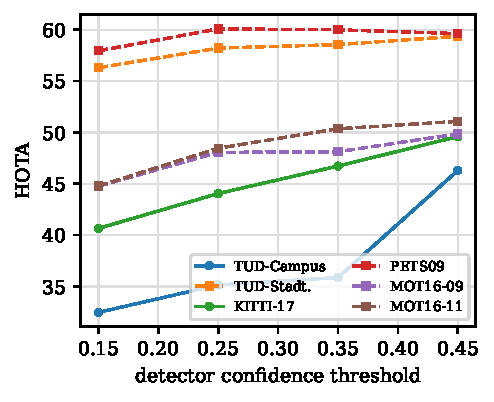
\includegraphics[width=\columnwidth]{figures/fig_hota_vs_conf.pdf}
\caption{HOTA vs.\ detector confidence threshold per video. Solid lines are the dense, low-precision
clips; on them HOTA rises as weak detections are filtered out.}
\label{fig:hota_vs_conf}
\end{figure}

\begin{figure}[t]
\centering
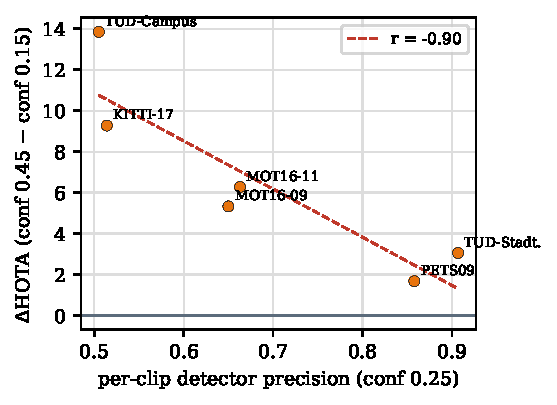
\includegraphics[width=\columnwidth]{figures/fig_money_plot.pdf}
\caption{The sign and size of recall's effect on HOTA (here, HOTA at conf~0.45 minus conf~0.15) track
per-clip detector precision: low-precision clips gain most from a higher confidence gate.}
\label{fig:money}
\end{figure}

\begin{figure}[t]
\centering
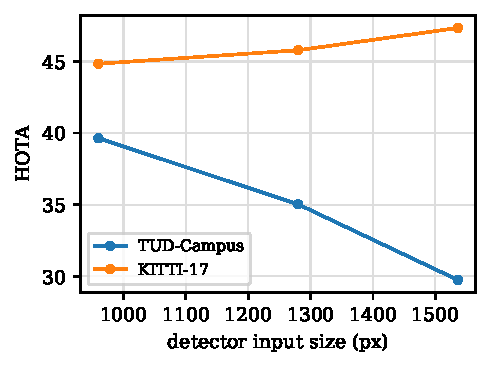
\includegraphics[width=\columnwidth]{figures/fig_imgsz_dense.pdf}
\caption{Input-size sweep on the two dense clips. Raising resolution (an orthogonal recall lever)
lowers HOTA, mirroring the confidence sweep.}
\label{fig:imgsz}
\end{figure}

\subsection{The Dropped Gate: a Restoration Ablation}
\label{sec:ablation}

To attribute the regression to the dropped gating contract rather than to the detector itself, we
restore the original DeepSORT gate -- $\text{min\_confidence}=0.3$ with NMS at overlap~$0.7$ -- on top
of the otherwise unchanged modern pipeline (\cref{fig:ablation}). Restoring the gate recovers HOTA on
the dense clips (mean $\ablationRecover$ HOTA on TUD-Campus and KITTI-17) while leaving the clean
clips essentially unchanged. Because the restored gate is the same confidence-plus-NMS filter the
original method applied, re-enabled by configuration alone, the recovered HOTA is causally
attributable to the gate.

\begin{figure}[t]
\centering
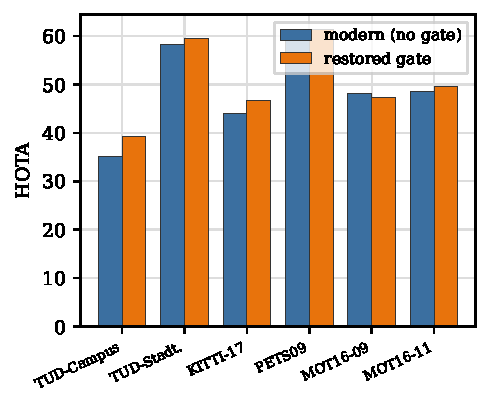
\includegraphics[width=\columnwidth]{figures/fig_ablation.pdf}
\caption{Gating-restoration ablation: per-video HOTA with the modern (ungated) pipeline vs.\ the
restored original confidence + NMS gate.}
\label{fig:ablation}
\end{figure}

\subsection{A Per-Clip Precision-Gating Guideline}
\label{sec:tuning}

The practical consequence is a simple per-clip policy: choose the detector confidence threshold from
the clip's precision regime rather than a single global default. Applied to the worst sequence,
raising the TUD-Campus threshold to $0.45$ moves it from a $\tudUntuned$ HOTA deficit (the global
default loses to the baseline there) to $+\tudGain$ over baseline, and the change is confined to that
sequence's preset, leaving the other five untouched. This single per-video override is what lifts the
modernized tracker to a win on all six videos in \cref{tab:fullpipeline}, at a mean real-time
throughput of \fpsRealtime{}~FPS.

\section{Limitations}
\label{sec:limitations}

Our evidence comes from six MOT-Challenge training-split videos
\cite{leal2015mot15,milan2016mot16}; there is no held-out test-split HOTA,
since the public benchmarks withhold test ground truth and we required it for
the per-clip detector-precision and association-isolation analyses. We
therefore report our findings as \textbf{per-clip and correlational rather
than as a universal law}: the link between low detector precision on dense,
low-resolution clips and the ``more detections hurt'' regime is consistent
across the sequences we audit (\cref{tab:detector,fig:money}), but six clips
cannot establish a calibrated precision threshold that transfers to arbitrary
domains. The practical guideline of \cref{sec:tuning} should be read as a
tuning heuristic, not a tuned constant.

A reviewer may object that restoring the original DeepSORT confidence and NMS
gate is ``self-inflicted'': we re-broke a filter the method already had, then
claimed credit for re-adding it. We address this head-on. The contribution is
not the gate itself but the \emph{audit} of what a routine modernization
silently discards: swapping in a modern detector and re-identification model
\cite{jocher2023yolov8,zhou2019osnet} quietly drops the gating contract, and
the resulting regression is invisible in mean HOTA yet large and predictable
per clip. The finding is also specific in mechanism. It concerns ungated
low-confidence detections \emph{instantiating spurious new tracks}, which is
distinct from ByteTrack \cite{zhang2022bytetrack}, where low-confidence boxes
are retained but only \emph{associated} to existing tracks and never seed new
ones. That distinction is what makes the result a property of the gating
contract rather than a tautology.

Detector and re-identification coverage is narrow. Two additional detector
backends, NanoDet and RTMDet, were unbuildable on our runtime (the NumPy-2.x
and ground-truth column-format issues noted in \cref{sec:method}), so the
detection-side claims rest on a single live detector and cannot speak to
cross-detector generality. Likewise the live pipeline uses one
re-identification family; the OSNet-versus-timm comparison
\cite{zhou2019osnet,wightman2019timm} isolates association only under
ground-truth boxes, so appearance robustness under real detections, and across
other re-identification architectures, remains untested. Confirming the
precision-gating guideline against modern DeepSORT descendants
\cite{du2023strongsort,cao2023ocsort,aharon2022botsort} on full benchmark
splits is left to future work.

\section{Conclusion}
\label{sec:conclusion}

We presented not a new tracker but an audit of an old one made new. Modernizing DeepSORT with a
contemporary detector and re-identification model lifts mean HOTA from \baselineHOTA{} to
\modernHOTA{} ($+\deltaHOTA$ tuned per clip; $+\deltaDefaultHOTA$ at the uniform default gate) at
\fpsRealtime{}~FPS end-to-end (timed on MOT16-09), a result that is by
itself unsurprising. The value lies in decomposing that gain and tracing its failure modes. The
improvement is detection-dominated rather than association-dominated, and on dense, low-resolution
clips the modernized pipeline can regress -- at its default gate it scores below the 2017 baseline on
the least-precise clip -- because it silently drops the original confidence and non-maximum-suppression
gate, letting ungated false positives instantiate spurious tracks. A gating-restoration ablation
partially recovers the loss (mean $\ablationRecover$ HOTA on the two dense clips), and the magnitude of
recall's effect on HOTA is anti-correlated with per-clip detector precision ($r = \corrPearson$, $n=6$).

The central takeaway is that, on these six clips, \textbf{per-clip precision gating is a
larger and more consistent HOTA lever than global recall maximization}. The practical guidance
follows directly: tune the detector confidence threshold per clip rather than trusting a single
global default, and when porting a legacy tracker to modern components, audit and explicitly
restore the gating contract instead of assuming the association core compensates. On the worst
sequence this moves the tracker from a $\tudUntuned$ deficit to $+\tudGain$ HOTA over baseline.

This audit is confined to six MOT-Challenge training videos and a single detector family. Future
work should validate the precision-gating guideline on held-out test sequences and across detector
families to establish that the effect is a property of tracking-by-detection rather than of
YOLOv8m, and should test whether an association-side gate in the spirit of ByteTrack and its
successors can recover low-confidence detections without reintroducing spurious tracks.


{\footnotesize
\bibliographystyle{ICICPEtran}
\bibliography{refer}
}

\end{document}
